%Đây là template dùng cho đề cương đề tài tốt nghiệp
%Khoa Công nghệ Thông tin
%Trường Đại học Khoa học Tự nhiên, ĐHQG-HCM

%Liên hệ về mẫu LaTEX này: Thầy Bùi Huy Thông (bhthong@fit.hcmus.edu.vn)

\documentclass{article}[14pt]
\usepackage[utf8]{vietnam}
\usepackage{enumerate}
\usepackage{enumitem}
\usepackage{multicol}
\usepackage{listings}
\usepackage[left=2cm,right=2cm,top=2.5cm,bottom=2.5cm]{geometry}
\usepackage{verbatim}
\usepackage{graphicx}
\usepackage{url}
\usepackage{fancyhdr}
\usepackage{fancybox,framed}
\linespread{1.3}
\usepackage{lastpage}
\usepackage{floatrow}
\usepackage{floatrow}
\pagenumbering{arabic}
%\pagestyle{fancy}
\newfloatcommand{capbtabbox}{table}[][\FBwidth]

\usepackage{blindtext}
\usepackage{titlesec}
\usepackage[nottoc]{tocbibind}
\usepackage{parskip}
\usepackage[table, svgnames, dvipsnames]{xcolor}
\usepackage{longtable}
\usepackage{makecell, cellspace, caption}
\newcolumntype{L}[1]{>{\raggedright\let\newline\\\arraybackslash\hspace{0pt}}m{#1}}
\newcolumntype{C}[1]{>{\centering\let\newline\\\arraybackslash\hspace{0pt}}m{#1}}
\newcolumntype{R}[1]{>{\raggedleft\let\newline\\\arraybackslash\hspace{0pt}}m{#1}}


\titleformat*{\section}{\LARGE\bfseries}
\titleformat*{\subsection}{\Large\bfseries}
\titleformat*{\subsubsection}{\Large\bfseries}
\setlength\parindent{0pt}
\setlength{\parskip}{5pt}

\begin{document}
    \begin{figure}[h]
        \begin{floatrow}
        \ffigbox{
\includegraphics[scale = .4]{images/logo.png}}  
        {%
    
        }
        \capbtabbox{
            \begin{tabular}{l}
            \multicolumn{1}{c}{\textbf{\begin{tabular}[c]{@{}c@{}}TRƯỜNG ĐẠI HỌC KHOA HỌC TỰ NHIÊN\\KHOA CÔNG NGHỆ THÔNG TIN\end{tabular}}} \\ \\ \\
            \end{tabular}
        }
        {%
    
        }
        \end{floatrow}
    \end{figure}
    
    \begin{center}
        
        %Xác định loại đề tài tốt nghiệp tương ứng: Khóa luận, Thực tập, Đồ án
        \textbf{\huge ĐỀ CƯƠNG KHOÁ LUẬN TỐT NGHIỆP} \\ 
    \end{center}
    
    %\vspace{.5cm}
    
    \begin{center}
    %Tên đề tài phải VIẾT HOA
        
        \textbf{\Large HỆ THỐNG DANH TIẾNG PHỤC VỤ XÁC THỰC HỒ SƠ VÀ ĐÁNH GIÁ KỸ NĂNG} 
        \\
        
    %Tên đề tài bằng tiếng Anh (nếu có)
    \vspace{.5cm}
        \textbf{\Large (Reputation system for résumé verification and skill assessment)}
    \end{center}
    
    \vspace{.5cm}
    
    \Large
    \section{THÔNG TIN CHUNG}
    \begin{itemize}[label = {}]
        
        \item \textbf{Giảng viên hướng dẫn:} 
        %Thể hiện dạng: <Chức danh> <Họ và tên> (<Đơn vị công tác>)
        \begin{itemize}
            PGS.TS. Nguyễn Đình Thúc (Trưởng Bộ môn Công nghệ tri thức)
        \end{itemize}{}
    
        
        \item \textbf{Nhóm sinh viên thực hiện:}
        
        %Thể hiện dạng: <Họ và tên sinh viên> (MSSV: )
        \begin{enumerate}
            \item Nguyễn Hải Tuyên (MSSV: 21127474) 
            \item Trần Minh Đạt (MSSV: 21127570)
        \end{enumerate}

       %Chọn loại thích hợp
        \item \textbf{Loại đề tài:} Ứng dụng
        
        \item \textbf{Thời gian thực hiện:} Từ 3/2025 đến 8/2025
        
        
    \end{itemize}
    
    \pagebreak 
    
    \section{NỘI DUNG THỰC HIỆN}
    {

    %Mỗi mục dưới đây phải viết ít nhất là 5 câu mô tả/giới thiệu.
    
    \subsection{Giới thiệu về đề tài}
    
    Phần này giới thiệu tóm tắt về đề tài và ngữ cảnh thực hiện (Nêu vấn đề, ý tưởng giải quyết, phương pháp giải quyết và ý nghĩa thực tiễn của vấn đề)
    
    %\textbf{Ghi chú:} Cần đăng ký tài khoản trên Overleaf\footnote{https://www.overleaf.com} và đọc cách sử dụng LaTeX tại hướng dẫn này \footnote{https://www.overleaf.com/learn/latex/Learn\_LaTeX\_in\_30\_minutes}% \cite{overleaf}.
    
    \subsection{Mục tiêu đề tài}
    
    %Phần này mô tả về động lực để giải quyết vấn đề. 
    Thông tin về bối cảnh của đề tài. Cần trả lời các câu hỏi:
    \begin{itemize}
        \item Tại sao cần thực hiện đề tài này?
        \item Đề tài mang lại được điều gì?
        \item Ảnh hưởng và ý nghĩa có thể có của kết quả đối với vấn đề đã được đặt ra nói riêng và toàn bộ hướng nghiên cứu nói chung?
    \end{itemize}
    
    \subsection{Phạm vi của đề tài}
    
    Nội dung nghiên cứu chính của đề tài. Các đối tượng nghiên cứu, thực thể liên quan, tập dữ liệu, ... có thể xuất hiện trong đề tài. Các giới hạn hoặc ràng buộc của đề tài. 
    
    \subsection{Cách tiếp cận dự kiến}
        %Có thể bổ sung hình ảnh vào để làm rõ phương pháp hoặc cách tiếp cận dự kiến.
        
        % Giới thiệu một số nghiên cứu (trong hoặc ngoài nước) đã được tiến hành theo hướng nghiên cứu của đề tài, nêu kết quả và nhận xét với các nghiên cứu này. Các trích dẫn từ các tài liệu sử dụng theo định dạng của tổ chức IEEE. Các ví dụ kế tiếp thể hiện trích dẫn tài liệu từ sách (\cite{latexcompanion}), từ bài báo trong tạp chí (\cite{einstein}) hay từ đường dẫn đến website (\cite{knuthwebsite}). \newline
        % Nêu các phương pháp, cách tiếp cận cũng như mô hình dự kiến thực hiện trong đề tài, chỉ rõ sự khác biệt (nếu có) so với các nghiên cứu đã được tiến hành ở trên.
        
        \subsubsection{Tổng quan về các nghiên cứu liên quan} 
            Trong phần này, chúng tôi sẽ trình bày tổng quan những nghiên cứu đã được tiến hành theo hướng nghiên cứu của đề tài hệ thống danh tiếng (Reputation System), bao gồm những nghiên cứu trong nước và những nghiên cứu ngoài nước. 
            \par
            % Nghiên cứu trong nước
            Đối với nghiên cứu trong nước, bài nghiên cứu "Quản Lý Định Danh Phi Tập Trung" của PGS.TS. Nguyễn Đình Thúc \cite{quan-ly-dinh-danh-phi-tap-trung} là xuất phát điểm quan trọng của đề tài. Ý tưởng chính của bài nghiên cứu là việc xây dựng một thống quản lý định danh số nơi người dùng (chủ thể định danh) có toàn quyền kiểm soát đối với thông tin định danh của mình, thay vì phụ thuộc vào các nhà cung cấp dịnh vụ (service provider). Bài nghiên cứu đã đề xuất việc sử dụng công nghệ chuỗi khối (blockchain) để xây dựng hệ thống định danh, bao gồm hai chủ thể chính: người dùng (chủ thể định danh) và nhà cung cấp dịnh vụ (service provider). Dữ liệu định danh của người dùng được lưu trữ cục bộ trên chính thiết bị của người dùng dưới dạng mã hóa và tham chiếu đến dữ liệu được lưu trên chuỗi khối (blockchain). Để quản lý dữ liệu mã hóa, cả chủ thể định danh và nhà cung cấp dịch vụ cần sử dụng giao thức tương tác DataTX. Chủ thể định danh có toàn quyền đối với dữ liệu của mình, có thể quản lý quyền truy cập thông qua giao thức tương tác AccessTx. 
            \par
            Bài nghiên cứu cũng đã định nghĩa về danh tiếng (reputation), hay uy tín như sau: "Uy tín được hình thành và biến đổi qua những thành công hay thất bại thực thể khi thực thi các nhiệm vụ cụ thể" \cite{quan-ly-dinh-danh-phi-tap-trung,a-survey-of-trust-in-internet-applications}. Có thể hiểu rằng, danh tiếng không phải là thực thể bất biến, mà luôn thay đổi theo thời gian và từng ngữ cảnh cụ thể. Không chỉ dừng lại ở một khái niệm lý thuyết đơn thuần, bài nghiên cứu đã đề xuất một hướng tiếp cận cụ thể để tính toán và số hóa khái niệm trừu tượng này bằng cách dựa vào hành vi (behavior) của các Node trong mạng, bao gồm người dùng (chủ thể định danh) và nhà cung cấp dịch vụ (service provider). Niềm tin của một thực thể (Node) được thiết lập là "giá trị kỳ vọng về hành vi tốt của Node trong tương lai" \cite{quan-ly-dinh-danh-phi-tap-trung}. Kỳ vọng này chính là xác xuất \(p\) trong phân phối Bernoulli, được tính bằng cách đếm số hành động của Node để tính xấp xỉ xác suất. \cite{thong-ke-may-tinh,quan-ly-dinh-danh-phi-tap-trung} 
            \par
            % Nghiên cứu ngoài nước
            Đối với các nghiên cứu ngoài nước, chúng tôi đã tham khảo từ các bài báo của dự án Rebooting the Web Of Trust (RWOT) như Portable Reputation Toolkit Use Cases \cite{reputation-toolkit}, Design Considerations for Decentralized Reputation Systems \cite{reputation-design}, và Reputation Interpretation \cite{reputation-interpretation}. Các bài báo trên đã đưa ra một khuôn khổ khái niệm (conceptual framework) cơ bản cho một hệ thống danh tiếng, đặc biệt trong việc đánh giá kỹ năng của một cá nhân khi tham gia vào mạng. 
            \par
            Bài báo Portable Reputation Toolkit Use Cases \cite{reputation-toolkit} đã đề xuất một quy trình chung gồm các bước thao tác của các thực thể trong một hệ thống danh tiếng:
            \begin{itemize}
                \item Mỗi cá nhân tham gia vào mạng bằng một mã định danh phi tập trung (DID - Distributed Identifier). 
                \item Chủ thể cần xây dựng danh tiếng sẽ tạo một tuyên bố (Assertion) và ký bằng khóa bí mật (private key) của mình. 
                \item Để tăng tính thuyết phục của tuyên bố (Assertion), chủ thể có thể tạo một bằng chứng (Evidence) và ký bằng khóa bí mật (private key) của mình, sau đó bổ sung tuyên bố ban đầu bằng cách tham chiếu đến bằng chứng vừa tạo.
                \item Các chủ thể khác tạo một bài đánh giá (Evaluation), ký bằng khóa bí mật của mình và tham chiếu đến tuyên bố (Assertion) của chủ thể cần xây dựng danh tiếng. Một bài đánh giá có thể ủng hộ (support) hoặc thách thức (challenge) tuyên bố gốc, có thể tham chiếu đến các bằng chứng (Evidence) để tăng tính thuyết phục. 
                \item Cộng đồng sẽ tham gia bình chọn cho các bài đánh giá. Họ có thể lựa chọn đồng tình hoặc không đồng tình với bài đánh giá. 
            \end{itemize}
            Bài báo Design Considerations for Decentralized Reputation Systems \cite{reputation-design} đã chỉ ra các yếu tố cốt lõi cần xem xét khi xây dựng một hệ thống danh tiếng phi tập trung, bao gồm bối cảnh (Context); sự tham gia của cộng đồng (Participation); sự đồng thuận của người dùng (User Consent); tính bảo mật (Confidentiality), khả năng tạo giá trị (Value Generation); hiệu suất hệ thống (Performance); tính bền vững của hệ thống (Sustainability); vòng đời của các tuyên bố (Claim Lifecycle); tính phục hồi sau các cuộc tấn công mạng (Resilience) và khía cạnh pháp lí (Legal). 
            \par
            Cuối cùng, bài báo Reputation Interpretation \cite{reputation-interpretation} đã tập trung vào việc tìm kiếm giải pháp để số hóa khái niệm trừu tượng danh tiếng. Danh tiếng của một chủ thể phụ thuộc vào rất nhiều yếu tố và ngữ cảnh khác nhau, vì vậy việc biến những dữ liệu thô đầu vào thành dữ liệu đầu ra nhất quán, có thể xử lý được (actionable output) là một phần quan trọng trong một hệ thống danh tiếng. Cụ thể hơn, bài báo đã đưa ra một quy trình tuần tự, bao gồm việc xác định dữ liệu đầu ra (output), xác định dữ liệu thô đầu vào (raw input), xác định chất lượng đầu vào và biên độ lỗi, chuẩn hóa dữ liệu để đưa về một dạng nhất quán, và cuối cùng là xử lý dữ liệu.
            \par
            Nhìn chung, các nghiên cứu, bài báo mà chúng tôi đã tham khảo từ trong và ngoài nước đã định hình một ý tưởng sơ khai về một hệ thống danh tiếng phi tập trung. Các nghiên cứu, bài báo đã đề xuất những quy trình xử lý, cách thức tương tác giữa các chủ thể trong hệ thống, kiến trúc hệ thống, cũng như các khía cạnh cần xem xét trong một hệ thống danh tiếng. Qua đó, đã tạo tiền đề cho bài nghiên cứu này về việc xây dựng và triển khai một hệ thống danh tiếng trong thực tiễn.  

        \subsubsection{Phương pháp và cách tiếp cận dự kiến}
            Dựa vào ý tưởng từ các nghiên cứu và bài báo đã tiến hành theo hướng đề tài này, chúng tôi đã nghiên cứu và thiết kế kiến trúc sơ bộ của hệ thống như hình \ref{fig:architect}. Hệ thống sẽ bao gồm các chủ thể tương tác sau: 
            \begin{itemize}
                \item \textit{Người đóng góp} (Contributor): Là những người dùng tạo các thử thách (Challenge), có trách nhiệm đóng góp ngân hàng thử thách của hệ thống.
                \item \textit{Người kiểm duyệt} (Moderator): Là những người có trách nhiệm kiểm duyệt các thử thách do người đóng góp tạo ra, thực hiện phân loại, đánh giá, và kiểm định chất lượng của thử thách. Để trở thành người kiểm duyệt, người dùng phải thõa mãn các điều điện cụ thể được quy định bởi hệ thống. 
                \item \textit{Người dùng chung} (Talent): Là những người có nhu cầu xây dựng danh tiếng, có thể tìm kiếm các thử thách, tham gia và đưa ra các giải pháp (Solution) tương ứng.
                \item \textit{Người đánh giá} (Reviewer): Là những người tham gia vào quá trình đánh giá giải pháp mà người dùng đưa ra cho một thử thách.
                \item \textit{Phòng tuyển dụng của các công ty} (Companies' recruitment department): Là đội ngũ tuyển dụng của các công ty có nhu cầu tuyển dụng những ứng viên phù hợp.
            \end{itemize}

            \begin{figure} [h!]
                \centering
                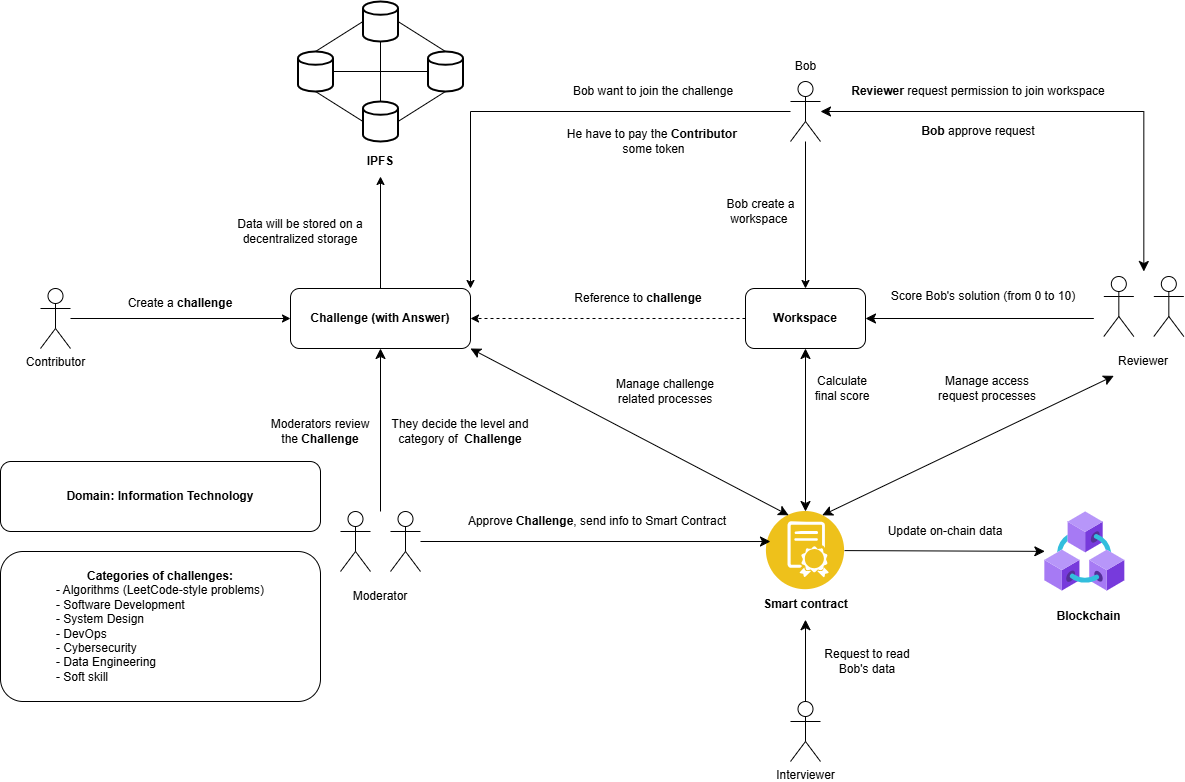
\includegraphics[width=0.97\textwidth]{images/prototype-v1.1.png}
                \caption{Kiến trúc hệ thống dự kiến}
                \label{fig:architect}
            \end{figure}

            \begin{enumerate}[label=\textbf{\alph*.}]
                \item \textbf{Các thành phần công nghệ chính:}
                \begin{itemize}
                    \item Blockchain: Sổ cái phi tập trung, có vai trò lưu trữ dữ liệu quan trong trên chuỗi (on-chain) như thông tin người dùng, danh sách thử thách, danh sách giải pháp, chỉ số danh tiếng, quyền truy cập vào dữ liệu của người dùng, \dots Dữ liệu có thể chứa các tham chiếu (CID) của các dữ liệu lưu ngoài chuỗi (off-chain). 
                    \item Smart Contract: Hợp đồng thông minh tương tác với blockchain để quản dữ liệu on-chain, đồng thời thực thi các tiến trình quan trọng như: tính toán chỉ số danh tiếng, cập nhật kết quả lưu trên chuỗi, thực hiện các biện pháp phạt theo quy ước. 
                    \item Dịch vụ lưu trữ dữ liệu phi tập trung: Giải pháp lưu trữ phi tập trung dùng để lưu trữ dữ liệu người dùng, nội dung của các \textit{thử thách} (Challenge), các \textit{giải pháp} (Solution) của nó, và các dữ liệu lớn cần lưu trữ ngoài khối (off-chain).
                \end{itemize}
                    
                \item \textbf{Kịch bản tương tác giữa các chủ thể:}
                \begin{itemize}
                    \item \textbf{Tạo thử thách:}
                    \begin{itemize}
                        \item Người đóng góp (Contributor) tạo và đăng tải các thử thách lên hệ thống. Nội dung của thử thách được lưu trữ và chia sẽ thông qua giao thức IPFS.
                        \item Mỗi thử thách thuộc một trong các phân loại: Thuật toán (Algorithm), Phát triển phần mềm (Software Development), Thiết kế hệ thống (System Design), DevOps, An toàn thông tin (Cyber Security), Kỹ năng mềm (Soft skills), v.v
                        \item Hệ thống lưu nội dung của thử thách ở kho lưu dữ liệu phi tập trung thông qua IPFS. Smart Contract cập nhật danh sách các thử thách trên chuỗi chứa các CID tham chiếu đến nội dung của thử thách ở IPFS.  
                        \item Các thử thách vừa tạo ở trạng thái chưa kiếm duyệt, cần phải thông qua ý kiến của những người kiếm duyệt (Moderator). 
                        \item Sau giai đoạn kiếm duyệt, nếu thử thách đạt mức độ và được hội đồng tán thành sẽ chuyển sang trạng thái đã kiểm duyệt. Những người cần xây dựng danh tiếng có thể tham gia vào thử thách. 
                    \end{itemize}

                    \item \textbf{Kiểm duyệt thử thách:}
                    \begin{itemize}
                        \item Những người kiểm duyệt (Moderator) đọc nội dung của thử thách, kiếm tra chất lượng và mức độ phù hợp của thử thách. Sau đó, những người kiểm duyệt tiến hành bỏ phiếu về các thông tin như: phân loại của thử thách, độ khó, mức độ phù hợp \dots
                        \item Smart Contract tổng hợp đánh giá của những Moderator, dựa trên một công thức tính đã quy định sẵn để tổng hợp ra kết quả cuối cùng. 
                        \item Smart Contract cập nhật thông tin liên quan của thử thách đã lưu trên chuỗi. 
                    \end{itemize} 

                    \item \textbf{Tham gia thử thách và đánh giá:}
                    \begin{itemize}
                        \item Người dùng (Bob) trả một khoản token nhất định cho Contributor để tham gia thử thách.
                        \item Hệ thống tự động tạo một không gian làm việc (workspace) nơi Bob có thể tạo giải pháp của mình. 
                        \item Bob thiết lập một phiên đánh giá bao gồm phần thưởng cùng số lượng tối đa Người đánh giá (Reviewer) có thể tham gia chấm điểm. Reviewer tham giá bằng cách tham gia vào workspace.
                        \item Sau khi hoàn thành đánh giá, mỗi Reviewer sẽ nộp điểm số kèm theo một khoản token đặt cược.
                        \item Smart Contract thu thập tất cả điểm số từ Reviewer, áp dụng thuật toán tính điểm để xác định số điểm cuối cùng.
                        \item Những Reviewer có điểm số gần với kết quả chính xác nhất sẽ nhận thêm token. Số lượng token đặt cược ban đầu càng lớn thì sẽ nhận lại càng nhiều. Reviewer có điểm số lệch xa với kết quả nhất (hoặc biên độ lệch vượt quá giới hạn đã quy định sẵn) sẽ bị phạt một lượng token dựa trên số token ban đầu đã đặt cược.  
                        \item Smart Contract sau đó cập nhật kết quả lên Blockchain để đảm bảo tính minh bạch và không thể chỉnh sửa.
                        \item Điểm số của giải pháp sẽ làm thay đổi chỉ số danh danh tiếng của người dùng trong một lĩnh vực cụ thể.
                    \end{itemize} 

                    \item \textbf{Chỉnh sửa giải pháp và cải thiện điểm:}
                    \begin{itemize} 
                        \item Người dùng (Bob) có thể cái thiện điểm bằng một trong hai cách: tạo thêm một phiên đánh giá cho giải pháp hiện tại hoặc cập nhật giải pháp và tạo một phiên đánh giá mới.
                        \item Quy trình tạo phiên đánh giá tương tự như phần trên.
                    \end{itemize} 

                    \item \textbf{Truy cập dữ liệu:}
                    \begin{itemize} 
                        \item Phòng tuyển dụng của các công ty có thể xem được chỉ số danh tiếng của Bob, những thử thách Bob đã tham gia, lịch sử số điểm đạt được tương ứng với giải pháp mà Bob đưa ra.
                        \item Để xem chi tiết các giải pháp của Bob, họ cần yêu cầu quyền truy cập vào workspace Bob.
                        \item Bob chấp nhận hoặc từ chối yêu cầu truy cập. 
                        \item Smart Contract cập nhật dữ liệu quyền truy cập lưu trên chuỗi. 
                        \item Phòng tuyển dụng xem xét và quyết định tuyển dụng đối với Bob. Nếu có, công ty cần trả một khoản token cho hệ thống. 
                    \end{itemize}
                \end{itemize}
            \end{enumerate}

        \subsubsection{Sự khác biệt so với các nghiên cứu trước}
            Bài nghiên cứu về hệ thống danh tiếng mà chúng tôi đang thực hiện thuộc hướng ứng dụng, với mục tiêu xây dựng và triển khai một hệ thống hoàn chỉnh dựa trên cơ sở lý thuyết của các bài nghiên cứu trong và ngoài nước đã được đề cập ở phần trên. Chính vì vậy, bài nghiên cứu này mang tính chất kế thừa, mang định hướng hiện thực hóa các ý tưởng được đề xuất từ các bài nghiên cứu mà chúng tôi đã tham khảo. 
    
    \subsection{Kết quả dự kiến của đề tài}
        Theo dự kiến, kết quả đầu ra của đề tài sẽ là một hệ thống hoàn chỉnh đảm bảo các yêu cầu: 
        \begin{itemize}
            \item Có giao diện tương tác người dùng hoàn chỉnh, đảm bảo thực hiện đầy đủ các chức năng theo yêu cầu. 
            \item Thành phần backend của hệ thống bao gồm các Smart Contract được kiểm thử chính xác và triển khai thành công. 
            \item Toàn bộ hệ thống có thể chạy được ở máy cục bộ với mục đích minh họa và có thể được triển khai trên một mạng chính của một blockchain (Polygon). 
        \end{itemize}
    
    \subsection{Kế hoạch thực hiện}
        Sau đây là bảng kế hoạch dự kiến cho tới hết tháng 6/2025.
        % Phần này mô tả về kế hoạch thực hiện (với các mốc thời gian tương ứng) cùng với việc phân chia công việc cho các thành viên tham gia đề tài. \textit{(Nên thể hiện dưới dạng bảng biểu)}

        \begin{longtable}{| C{4cm} | L{7cm} | L{5cm} |}
            \hline
            \rowcolor{Gainsboro!60}
            \makecell{Mốc thời gian} & \makecell{Công việc} & \makecell{Phân công}\\
            \hline
            \endhead
            01/02/2025 
            & Tìm hiểu các công nghệ lập trình ứng dụng phân tán (dApp) như ngôn ngữ lập trình Solidity; khung lập trình Hardhat; các công nghệ chuỗi khối tiềm năng có mức chi phí hợp lí; thư viện hỗ trợ tương tác với chuỗi khối như wagmi, viem, v.v; dịch vụ ví điện tử hỗ trợ tích hợp với dApp như Metamask, CoinBase, v.v; dịch vụ lưu trữ phi tập trung IPFS, Irys, Arweave.  
            & Nguyễn Hải Tuyên, Trần Minh Đạt \\
            \hline
            01/03/2025 
            & Vẽ kiến trúc hệ thống sơ bộ, mô tả các thành phần cần thiết trong hệ thống, các luồng hoạt động chính của hệ thống cũng như các thành phần công nghệ cần thiết. 
            & Trần Minh Đạt \\
            \hline
            08/03/2025 
            & Xây dựng kịch bản tương tác giữa các chủ thể trong hệ thống.
            & Nguyễn Hải Tuyên \\
            \hline
            18/03/2025 
            & Khởi tạo dự án, cài đặt các thư viện, khung lập trình cần thiết.
            & Trần Minh Đạt \\
            \hline
            27/03/2025 
            & Hoàn thiện tính năng đăng nhập, người dùng có thể sử dụng ví điện tử cài đặt sẵn trên trình duyệt để đăng nhập vào hệ thống.
            & Nguyễn Hải Tuyên \\
            \hline
            01/04/2025 
            & Lập trình quản lý thông tin người dùng trong hệ thống, một người dùng cần đảm các thông tin như tên, email, mô tả, v.v. Cần đảm bảo tên người dùng là duy nhất trong hệ thống. Nghiên cứu xây dựng một hợp đồng thông minh quản lý thông tin của người dùng. Xây dựng kiểu dữ liệu User với các trường thông tin cần thiết. Đồng thời, nghiên cứu xây dựng các phương thức cần thiết cho việc truy vẫn, cập nhật và xóa dữ liệu. Tích hợp sử dụng dịch vụ lưu trữ phi tập trung như IPFS, Irys, Arweave, v.v đối với các dữ liệu lớn. Bên cạnh đó, sử dụng NextJS để xây dựng giao diện tương tác với người dùng. 
            & Nguyễn Hải Tuyên \\
            \hline
            08/04/2025 
            & Hoàn thiện các chức năng của người đóng góp (Contributor) cho phép tạo, chỉnh sửa hoặc xóa các thử thách. Nghiên cứu xây dựng một hợp đồng thông minh quản lý các thử thách trong hệ thống. Xây dựng một kiểu dữ liệu phù hợp cho thử thách và triển khai các phương thức cần thiết. Bổ sung các trường thông tin của người dùng về các thử thách mà họ đã tạo. 
            & Trần Minh Đạt \\
            \hline
            15/04/2025 
            & Hoàn thiện các chức năng của kiếm duyệt (Moderator) cho phép đọc dữ liệu và đánh giá. Xác định trường thông tin cần thiết mà người kiếm duyệt cần phải hoàn thiện trước khi nộp biểu quyết. Nghiên cứu và triển khai cơ chế tổng hợp ý kiến của tất cả những người kiểm duyệt. Xây dựng một công thức tính hiệu quả, xác định các trọng số phù hợp như chỉ số danh tiếng, v.v 
            & Nguyễn Hải Tuyên \\
            \hline
            30/04/2025 
            & Hoàn thiện chức năng của người dùng chung cần xây dựng danh tiếng, cho phép họ tham gia vào các thử thách. Triển khai một không gian riêng của người dùng cho phép người dùng trình bày giải pháp của mình. Bổ sung giao diện tương tác phù hợp về phía frontend.
            & Trần Minh Đạt \\
            \hline
            10/05/2025 
            & Nghiên cứu xây dựng một hợp đồng thông minh triển khai một đồng tiền chung cho hệ thống, token sử dụng phải đảm bảo tuân theo các tiêu chuẩn của ERC20 \cite{ERC20}. 
            & Nguyễn Hải Tuyên \\
            \hline
            20/05/2025 
            & Hoàn thiện các chức năng của người đánh giá (Reviewer), cho phép họ xem chi tiết giải pháp khi tham gia vào không gian làm việc của người tạo ra giải pháp. Nghiên cứu xây dụng công thức tính số điểm cuối cùng tổng hợp từ các đánh giá của Reviewer, công thức phải tính đến các trọng số quan trọng như chỉ số danh tiếng của từng Reviewer. Nghiên cứu triển khai cơ chế đặt cược, thưởng và phạt sau khi tổng hợp được kết quả cuối cùng.  
            & Trần Minh Đạt \\
            \hline
            01/06/2025 
            & Hoàn thiện chức năng của các phòng tuyển dụng của các công ty, cho phép họ tìm kiếm hồ sơ của người dùng. Xác định những thông tin nào được công khai theo mắc định, những thông tin nào cần phải có sự đồng ý của người dùng mới có thể truy cập. Nghiên cứu cơ chế trả phí khi các phòng tuyền dụng xác nhận tuyển ứng cử viên.  
            & Nguyễn Hải Tuyên \\
            \hline
            20/06/2025 
            & Viết mã nguồn kiểm thử hoàn chỉnh, thực hiện kiểm thử tất cả các tính năng của hệ thống, đảm bảo hệ thống hoạt động ổn định.   
            & Trần Minh Đạt \\
            \hline
            30/06/2025 
            & Xử lý các lỗi hệ thống phát hiện được thông qua quá trình kiểm thử, đảm bảo hệ thống hoạt động chính xác.   
            & Nguyễn Hải Tuyên, Trần Minh Đạt \\
            \hline
        \end{longtable}
    }
    
    \pagebreak 
    %TÀI LIỆU TRÍCH DẪN
    %Đây là ví dụ
    \bibliographystyle{ieeetr}
    \bibliography{reference}
    \nocite{*}

    \begin{table}[h]
    \centering
        \begin{tabular}{p{7cm}p{7cm}}
        \textbf{
            \begin{tabular}[c]{@{}c@{}}\\XÁC NHẬN CỦA GVHD\\ \textit{(Ký và ghi rõ họ tên)}\end{tabular}} 
            & \textbf{\begin{tabular}[c]{@{}c@{}}\textit{Tp. Hồ Chí Minh, ngày... tháng... năm...}\\NHÓM SINH VIÊN THỰC HIỆN\\\textit{(Ký và ghi rõ họ tên}) \end{tabular}}
        \end{tabular}
    \end{table}
    
\end{document}


